\section{Implementation Details of the Algorithm Extracting Semantically Meaningful Tokens} \label{app:new_method}

In \Cref{fig:algo_python} we give the algorithmic implementation of the classification of semantically meaningful tokens as defined in \Cref{sec:new_method} for the python list style function call outputs by the models \texttt{qwen/qwen2.5-\{0.5,3,7\}B-instruct}, \texttt{qwen/qwen3-4B-instruct-2507}, \texttt{google/gemma-2-9b-it} as well as \texttt{google/gemma-3-\{4,12\}b-it}.
In \Cref{fig:algo_json}, we do the same for the JSON-style function call outputs by
\texttt{mistralai/} \texttt{Ministral-8B-Instruct-2410}.



\begin{figure*}[htb]
\centering
    \begin{subfigure}[c]{0.99\textwidth}
        \centering
        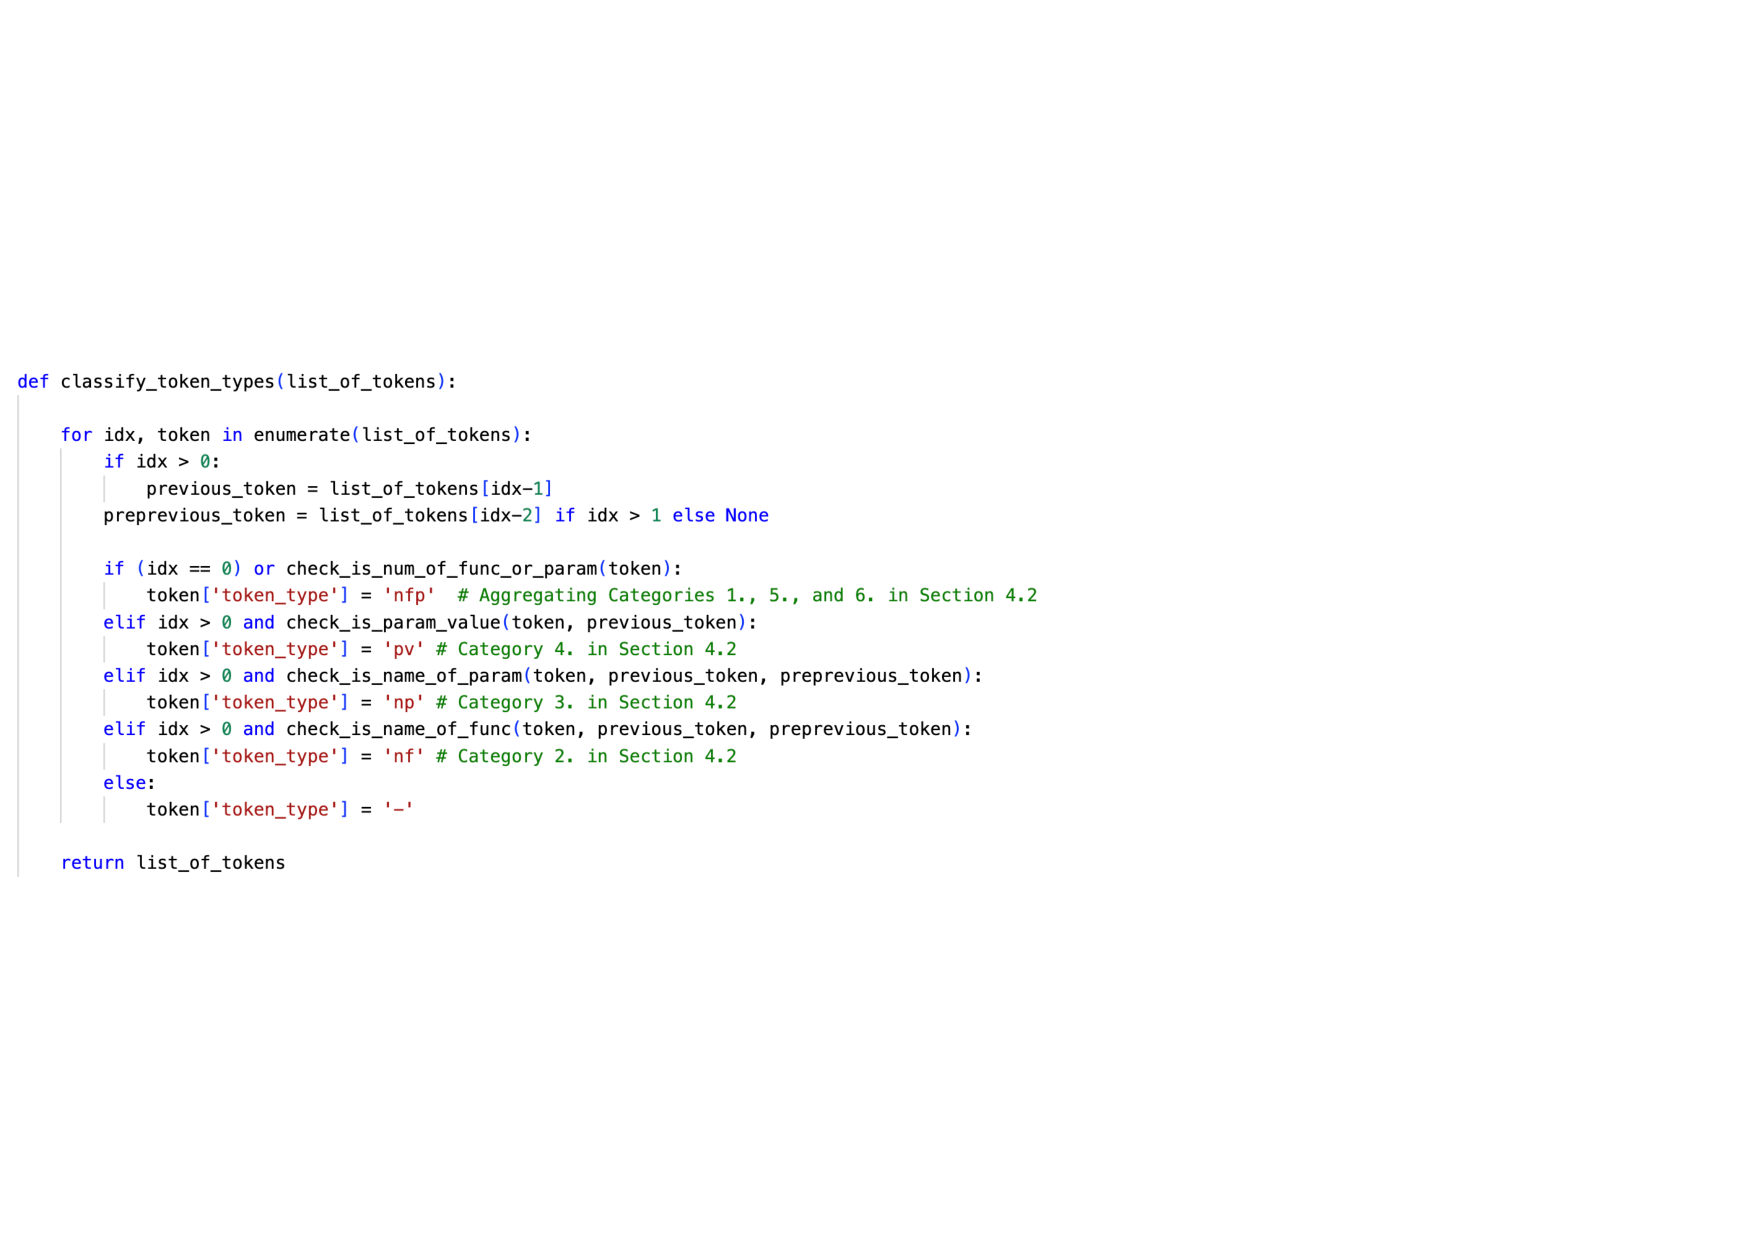
\includegraphics[width=\textwidth]{figures/AlgoPythonP1.pdf}
        
        \caption{The overall algorithm for classifying the tokens in a sequence of tokens.}
        \label{fig:algo_python_p1}
    \end{subfigure}
    
    \begin{subfigure}[c]{0.99\textwidth}
        \centering
        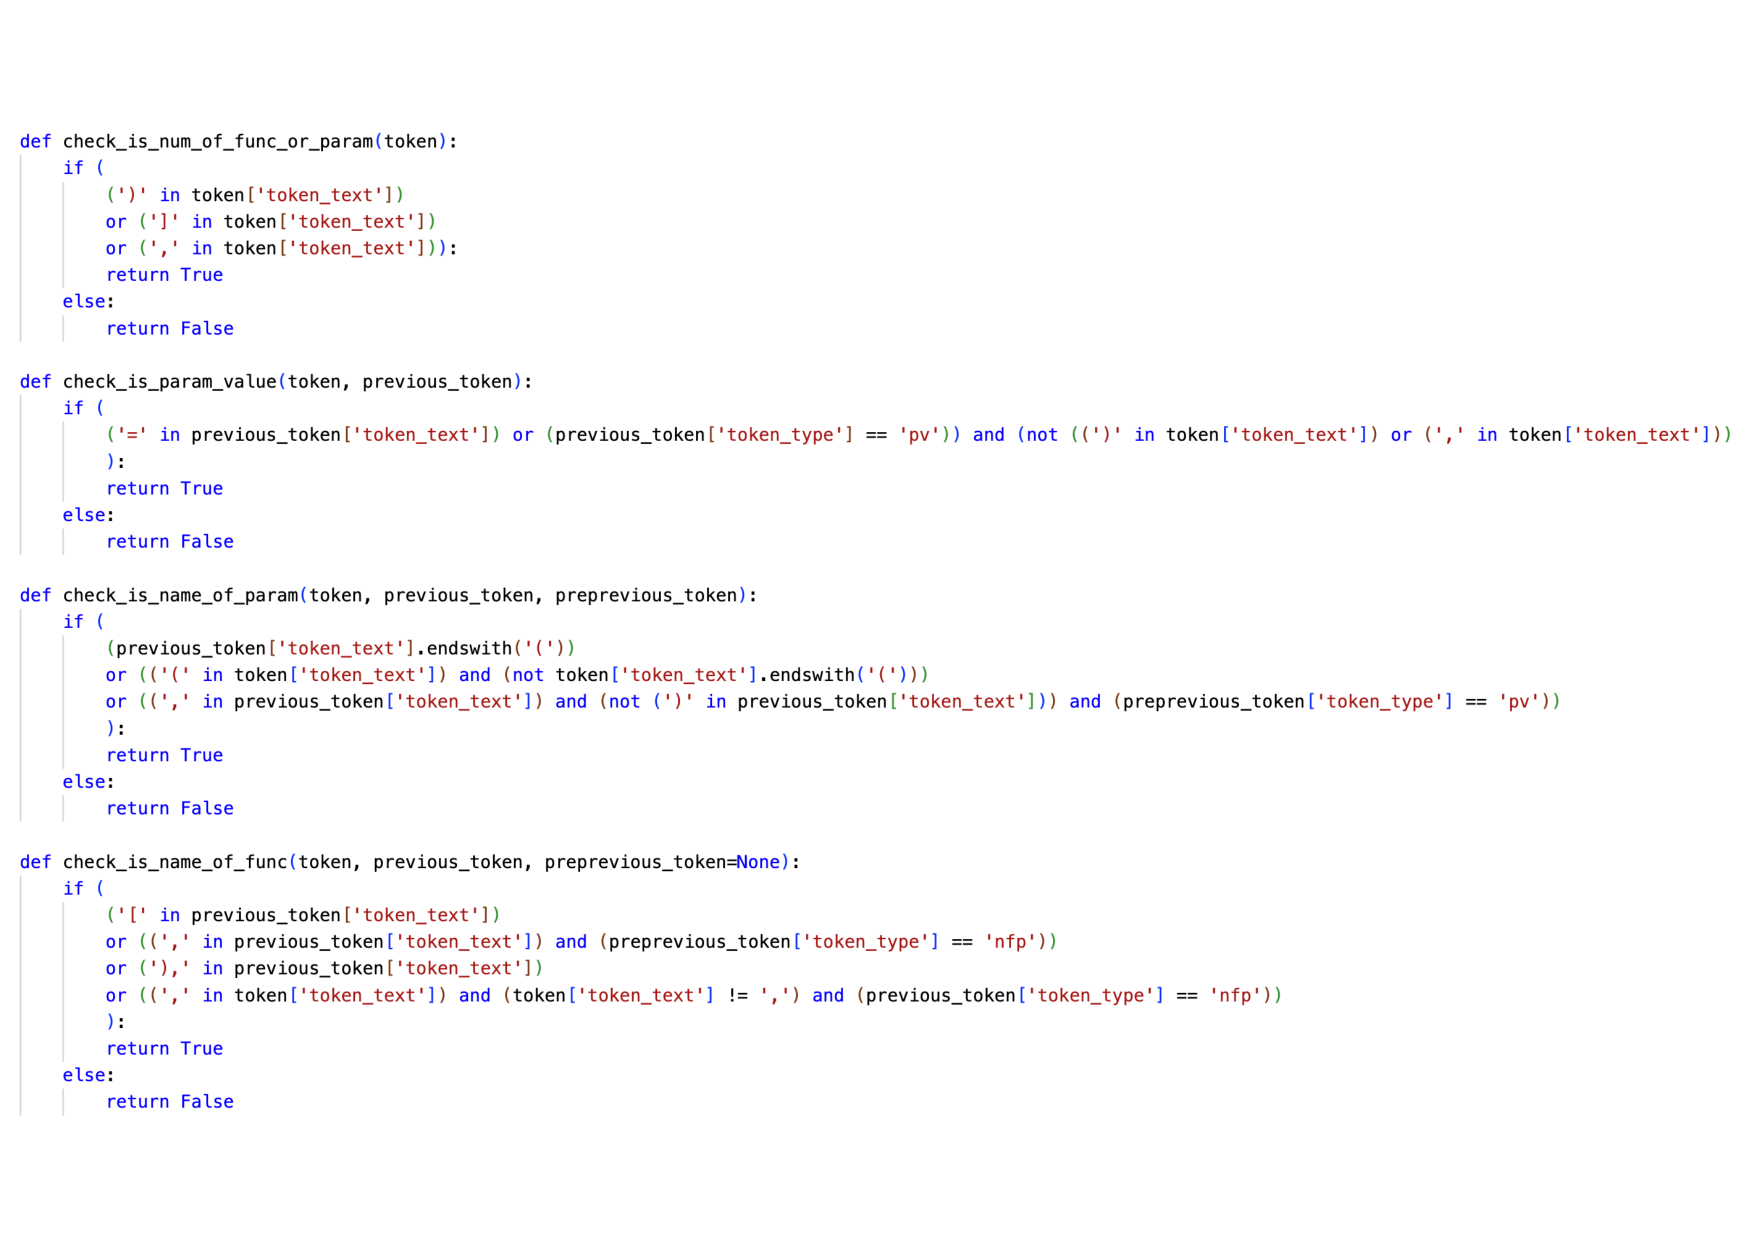
\includegraphics[width=\textwidth]{figures/AlgoPythonP2.pdf}
        \caption{The individual token classification functions.}
        \label{fig:algo_python_p2}
    \end{subfigure}

    \caption{
        The algorithmic implementation of the classification of semantically meaningful tokens as defined in \Cref{sec:new_method} for the python list style function call outputs by the models \texttt{qwen/qwen2.5-\{0.5,3,7\}B-instruct}, \texttt{qwen/qwen3-4B-instruct-2507}, and \texttt{google/gemma-2-9b-it} as well as \texttt{google/gemma-3-\{4,12\}b-it}.
    }
    \label{fig:algo_python}
\end{figure*}



\begin{figure*}[htb]
\centering
    \begin{subfigure}[c]{0.99\textwidth}
        \centering

        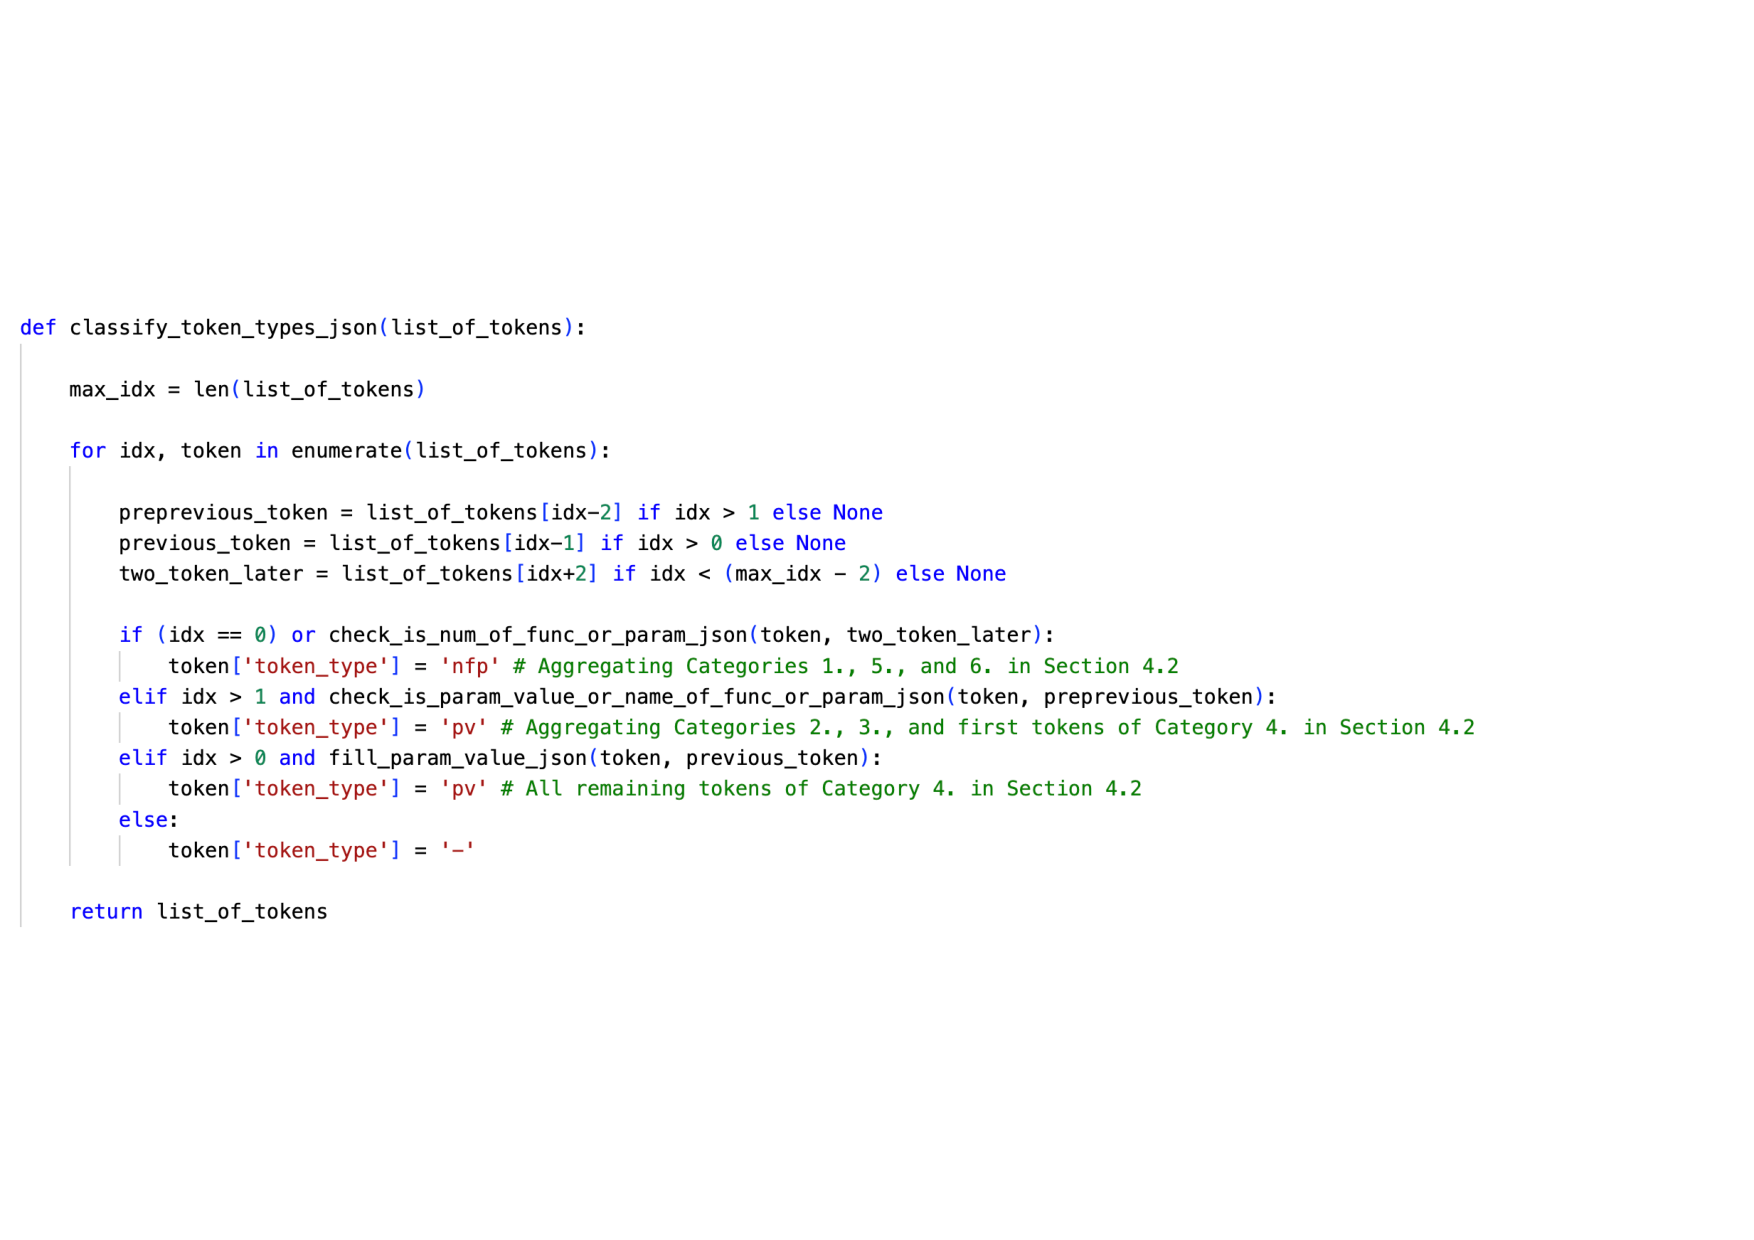
\includegraphics[width=\textwidth]{figures/AlgoJSONP1.pdf}
        \caption{The overall algorithm for classifying the tokens in a sequence of tokens.}
        \label{fig:algo_json_p1}
    \end{subfigure}
    \begin{subfigure}[c]{0.99\textwidth}
        \centering
        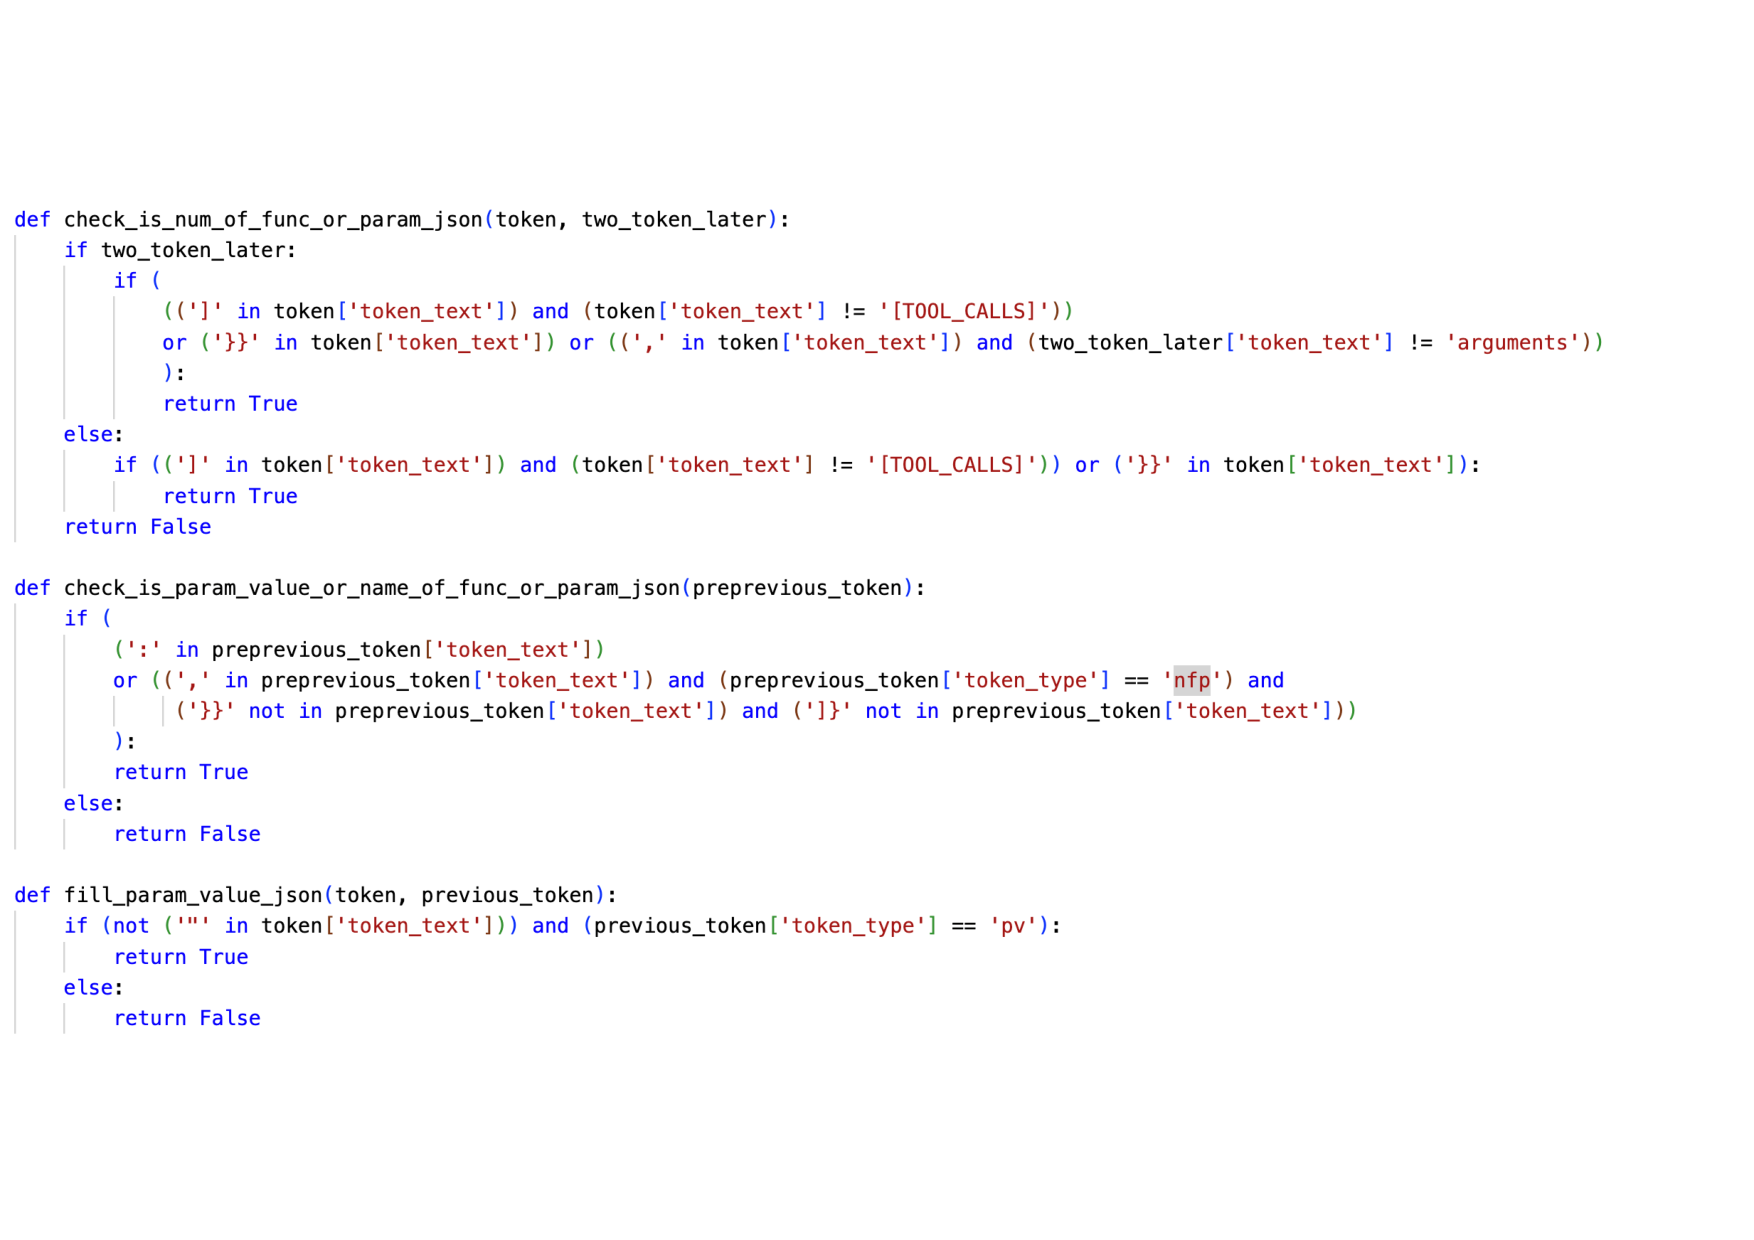
\includegraphics[width=\textwidth]{figures/AlgoJSONP2.pdf}
        \caption{The individual token classification functions.}
        \label{fig:algo_json_p2}
    \end{subfigure}

    \caption{
        The algorithmic implementation of the classification of semantically meaningful tokens as defined in \Cref{sec:new_method} for the JSON-style function call outputs by \texttt{mistralai/} \texttt{Ministral-8B-Instruct-2410}.
    }
    \label{fig:algo_json}
\end{figure*}





\begin{algorithm*}[t]
\caption{SMT typing for Python-call tool outputs}
\label{alg:smt-python}
\begin{algorithmic}[1]
\REQUIRE Token list $T=[t_0,\dots,t_{N-1}]$, each token has \texttt{token\_text}
\ENSURE Same tokens with \texttt{token\_type} $\in \{\texttt{nfp},\texttt{nf},\texttt{np},\texttt{pv},\texttt{-}\}$

\FOR{$i \leftarrow 0$ \TO $N-1$}
  \STATE $t \leftarrow T[i]$
  \STATE $t^{-1} \leftarrow T[i-1]$ \textbf{if} $i>0$ \textbf{else} \texttt{None}
  \STATE $t^{-2} \leftarrow T[i-2]$ \textbf{if} $i>1$ \textbf{else} \texttt{None}

  \IF{$i=0$ \OR $\textsc{IsSeparatorOrCloserPython}(t)$}
    \STATE $t.\texttt{token\_type} \leftarrow \texttt{nfp}$
  \ELSIF{$i>0$ \AND $\textsc{IsParamValuePython}(t, t^{-1})$}
    \STATE $t.\texttt{token\_type} \leftarrow \texttt{pv}$
  \ELSIF{$i>0$ \AND $\textsc{IsParamNamePython}(t, t^{-1}, t^{-2})$}
    \STATE $t.\texttt{token\_type} \leftarrow \texttt{np}$
  \ELSIF{$\textsc{IsFuncNamePython}(t, t^{-1}, t^{-2})$}
    \STATE $t.\texttt{token\_type} \leftarrow \texttt{nf}$
  \ELSE
    \STATE $t.\texttt{token\_type} \leftarrow \texttt{-}$
  \ENDIF
\ENDFOR

\STATE \textbf{return} $T$
\end{algorithmic}
\end{algorithm*}






